\chapter{Introduction}
\label{sec:introduction}
When designing systems, most developers face a two-fold challenge of finding a common fashion of expressing the system and its components so that it is both understandable for people outside the software engineering world, and at the same time gives both a low- and high-level description of the system for the purpose of development. Many methods have been designed to solve this, one of which is the \bon{} method. \bon{} relies on both graphical and textual elements. When developing Eiffel in EiffelStudio, the user has a graphical \bon{} tool available, which he can quickly open for a graphical overview of inheritance and client relations of a given class. Furthermore, there is no tool for inspecting the textual aspect of \bon. If one wants a textual representation they must write it by hand themselves.

\section{The Business Object Notation}
The Business Object Notation (\bon{}) is a specification language and notation for writing software specifications defined by Kim Wald\'en and Jean-Marc Nerson in their book \textit{Seamless Object-Oriented Architecture: Analysis and Design of Reliable Systems} \cite{walden1995}. \bon{} is based on the principles of reusability, seamlessness, and reversibility, along with software contracting. Reusability refers to the idea of reducing the complexity of a system by relying on reusable components, while at the same time keeping the specifications created in \bon{} at an abstraction level that enables other developers to benefit from one's work. Seamlessness is based on the notion of seamless transition between requirement specification, analysis, design, and implementation. Reversibility concerns the idea that for a software specification to have any value, changes in implementation must always be reflected back on the specification and vice versa.

\bon{} has two parts; a graphical notation and a textual notation. While this project focuses on textual \bon{}, the graphical notation is used to present object structures and hierarchies throughout the report. Below is a simple example of graphical \bon{}:

\begin{figure}[H]
    \centerline{\scalebox{0.7}{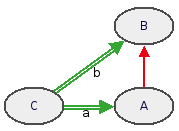
\includegraphics{images/graphical-bon-example.png}}}
    \caption[Example of the graphical \bon{} notation]{Example of the graphical \bon{} notation. Red arrows denote inheritance relations, while green double arrows denote client-supplier relations.}
    \label{fig:context-classes}
\end{figure}

In particular, the motivation behind this project is aimed at adding seamlessness and reversibility to EiffelStudio by adding seamless switching between Eiffel source code and textual \bon{}, which by consequence will lead to reversibility.

\paragraph{}
The grammar for the textual \bon{} notation is defined on pages 352-359 in the aforementioned book \cite{walden1995}, and this report relies heavily on this grammar and the keywords and ideas that it introduces.

\section{Reading Guide}
This report is primarily addressed to readers with a quite thorough understanding of \bon{} and the general ideas of object-oriented design. Readers with no or only little prior exposure to \bon{} will benefit greatly from keeping a copy of \textit{Seamless Object-Oriented Architecture} for reference while reading.\footnote{As the book is currently out of print, a PDF copy can be obtained from \textit{http://www.bon-method.com/}}. Even readers well versed in the ideas of \bon{}, but not in the syntax of the textual notation, will find the previously mentioned definition of the grammar to be helpful.

Aside from \bon{}, the reader is assumed to a have solid understanding of basic programming concepts, specifically object-orientation and imperative programming style. Seeing as the products of this project is written in the Eiffel programming language\footnote{For further information, see http://www.eiffel.com/}, the following terms should be fully understood by the reader:
\begin{itemize}
\item \textit{feature} --- corresponds to what is commonly denoted as a \textit{method} in other imperative languages such a Java and C\#.
\item \textit{attribute} --- corresponds to the term \textit{field}
\item \textit{agent} --- agents wrap actions into objects, and correspond to the notion of an \textit{anonymous inner class} in Java, a \textit{delegate} in C\#, and the idea of a closure in functional programming
\item \textit{attached} --- if a feature is attached, it refers to the fact that a reference must be associated with an object (i.e. not refer to \textit{Void})
\end{itemize} 

\subsubsection{Outline}
Chapter 1 (this chapter) presents a definition of the problem that this project aims to solve alongside basic knowledge for further understanding notions presented later on.
\paragraph{}
Chapter 2 describes the background for the project as well as many of the design decisions on which the implementations presented in later sections are based.
\paragraph{}
Chapter 3 unfolds the specifics of how textual \bon{} has been integrated into EiffelStudio.
\paragraph{}
Chapter 4 discusses the implementation of a general-purpose type checker for textual \bon{}, in particular how the restrictions on the grammar are implemented.
\paragraph{}
Chapter 5 lays out a number of possibilities for further development of the work initiated by this project.
\paragraph{}
Chapter 6 contains a conclusion on the findings in the remainder of the report.

\section{Problem Definition}
The purpose of this project is to bridge the gap between textual \bon{} and EiffelStudio by providing a way to statically extract textual \bon{} from Eiffel source code within the EiffelStudio environment. It should be easy to quickly switch from editing Eiffel source code to viewing textual \bon. Furthermore, a textual \bon{} type checker must be able to check the well-typedness of the extracted \bon{} and return an appropriate error message to the user when it is not. It should be implemented in such a way that it in the future can be inserted into EiffelStudio. The final product must:
\begin{itemize}
  \item Provide a way to view textual \bon{} within the EiffelStudio environment
  \item Add syntax highlighting for textual \bon{}
  \item Provide a way to extract textual \bon{} in EiffelStudio
  \item Implement a type checker for textual \bon{} 
\end{itemize}
To achieve the first part, the EiffelStudio environment will be analyzed and discussed in chapters 2 and 3. The analysis is based on similar functionality already existing in EiffelStudio. In particular, it is studied how EiffelStudio currently provides functionality for viewing Eiffel source code from different perspectives.

For the second part, based on further analysis of EiffelStudio, a syntax highlighting mechanism for textual \bon{} is examined based on the syntax highlighting already done for Eiffel. 

Textual \bon{} extraction will be discussed in chapter 3 as an extension of aforementioned way of displaying textual \bon. The goal is for the extractor to provide a meaningful overview over an Eiffel system with textual \bon{}.

Finally, chapter 4 contains a discussion of a textual \bon{} type checker and how it is implemented. Important design decisions and interesting challenges are explained.

\section{The Product}
Writing specifications can be a strain, thus many of developers want to shortcut this work by generating the specification with tools. However, as mentioned above, there are no tools to extract \textsc{bon} from Eiffel, even thought \bon{} originates from the world of Eiffel. Doing so, is the exact purpose of this tool. A tool to extract Eiffel from \textsc{bon}, in the main Eiffel development environment, EiffelStudio. The idea is that a user at any given time can switch from writing Eiffel code, to reading a textual \bon{} specification for his work. Still, the extracted \bon{} should not just analyze one class, but also provide an overview of other relations of the class.

To ensure that the extracted textual \bon{} is syntactically correct and well-typed, a type checker is also implemented. This type checker will receive the \bon{} through an extended version of the \textsc{ebon} parser/lexer (\cite{ebon}). A this point this type checker is not yet integrated in EiffelStudio, but as it is fully implemented in Eiffel, it is the next logical step. 

\section{Related Work}

\subsubsection{Extended BON}
The Extended \bon{} Tool Suite (\textsc{ebon}) is a project whose objective is to add semantic properties into the \bon{} standard. Extended \bon{} is developed by Joseph Kiniry. The textual \bon{} parser and lexer used for the work described in this report is based on the parser and lexer from \textsc{ebon}, as well the abstract syntax as a meta object graph.

\subsubsection{BONc}
\bon{c} is a command-line textual \bon{} parser and type checker implemented in Java \cite{bonc}. The tool is developed and maintained by Fintan Fairmichael. \bon{c} provides support for generating graphical representations of a \bon{} specification, namely through generation of informal charts in HTML format and graphical \bon{} diagrams. The standard types defined in the type checker described in the report is based in the built-in types in \bon{c}.

\subsubsection{BON IDE}
The \bon{} Integrated Development Environment is a tool which puts emphasis on the graphical aspect of \bon{} \cite{bonide}. It provides tool for visualizing a \bon{} specification as a graphical diagram, and bases its work on the Ecore model of \bon{}.

\subsubsection{The BON CASE Tool}
The BON CASE Tool is a CASE (Computer-Aided Software Engineering) tool that supports the creation of \bon{} models and the formal reasoning of such \cite{boncase}. It supports integration of \bon{} with \textsc{jml} in order to be able to utilize the formal techniques and tools of \textsc{jml}. The BON CASE Tool is developed by Paige, Kaminskaya, Ostroff, and Lancaric.

\subsubsection{Other Papers}
\cite{ostroff2001} formulates a metamodel for \bon{} using PVS, which expresses the syntactic constraints that all models using \bon{} must obey. Some of the rules defined here have been implemented in the type checker described in this report.

\cite{ostroff1999} describes how the properties of \bon{} make the language a well suited tool for formal specifications and algorithm refinement.

\cite{ostroff1998} shows how a transition from the \textsc{z} formal notation to \bon{} can be made. Furthermore, Paige and Ostroff show how \bon{} has the expressive power of \textsc{z} with the added value of an object-oriented approach.

\import{./}{ack}